%%=============================================================================
%% Uitwerking
%%=============================================================================

\chapter{Uitwerking}
\label{ch:uitwerking}


\section{Benodigdheden}
\label{sec:Benodigdheden}

\subsection{Data}
Een onmisbaar onderdeel om aan machine learning te doen is uiteraard de data. Tijdens de eerste fases van het project wordt er gebruik gemaakt van zelfgegenereerde data in Excel. De data die uit de arcademachine ontvangen zal worden zal in csv-formaat zijn. Doordat Excel-tabbladen opgeslagen kunnen worden in een csv-file is dit dan ook een logische keuze. 
Er zullen zo'n 400 metingen beschikbaar zijn die kunnen ingelezen worden in het programma. 

We willen uiteraard weten hoe goed het algoritme scoort dit kunnen we testen door testdata te voorzien. De dataset die we uit Excel halen zal opgesplitst worden in trainingsdata en testdata. Het algoritme zal met de trainingsdata een hypothese vormen die ervoor zal zorgen dat ook nieuwe of nog ongekende data een goede voorspelling krijgt. Daarom is het belangrijk om een dataset te hebben die data bevat die nog niet eerder gebruikt is door het algoritme. Enkel op deze manier kunnen we zeker zijn dat het algoritme een goede hypothese heeft gemaakt. 

\subsection{Frameworks}
Zoals in de inleiding reeds besproken was zijn er verschillende soorten frameworks die reeds geïmplementeerde algoritmen hebben. Een eerste mogelijk framework was TensorFlow van Google. Dit is ontwikkelt in Python, de algoritmen die hierin voorzien zijn zijn voornamelijk neurale netwerken of deep learning algoritmen. Het is mogelijk om ook eenvoudigere algoritmen te gebruiken maar daar ligt de specialiteit niet op. En dit in combinatie met een taal die ik niet machtig ben lijkt mij geen goede keuze. Er zijn nog een aantal andere frameworks die gemaakt zijn in andere programeertalen zoals Javascript, Node.js, Java, etc. 

Accord-framework is daar een van, dit is ontwikkelt in .NET. Alle algoritmen die nodig zijn om deze bachelorproef tot een succesvol einde te brengen zijn beschikbaar. \newline
Doozekerr te werken met het Accord-framework bestaat er een mogelijk om in de toekomst een webapplicatie te ontwikkelen. Dit openend dus ook nog extra mogelijkheden om te experimenteren met Artificiële Intelligentie. 
\newline
.NET is een nog niet zo'n populaire taal om aan artificiele intelligentie te doen maar er zit potentieel in. Doordat .NET vele gelijkenissen heeft met Java is er een nog groter publiek die hiermee aan de slag kan.
\newline
Door deze mogelijkheden lijkt dit dan ook het meest geschikte framework om aan het werk te gaan. 

\section{Fase 1}
\label{sec:Fase1}
De eerste stap om een programma te maken om voorspellingen te doen is de data maken. Omdat dit ook nog maar de eerste fase is beginnen we gemakkelijk. Dit wil zeggen dat we de computer een eerste voorspelling laten doen tussen twee totaal verschillende spelletjes. We nemen Pac-man en Mortal Combat (schietspel) om te starten. Pac-man kan gespeeld worden enkel d.m.v. joystickbewegingen. Om Mortal-Combat te spelen heb je veel de knoppen nodig maar ook de joystick.  Nu als mens is het gemakkelijk om dit verschil te kunnen zien, als er knoppen gebruikt geweest zijn was de speler Mortal-Combat aan het spelen. 

\subsection{Data}
\label{sec:DataFase1}
De eerste dataset is zelf gegenereerd zonder echte input van de arcademachine omdat het systeem die de data zal inlezen nog in ontwikkeling is op dit moment. 
In Excel zijn er drie kolommen voorzien een kolom voor het aantal keer dat de knoppen ingedrukt zijn geweest gedurende twee minuten. Dan het aantal keer dat de joystick bewogen is in diezelfde tijdsspanne. De derde kolom staat het ID van het spel. 
In figuur \ref{fig:regressieFig} ziet u random 10 voorbeelden uit de dataset.
Het GameID 0 wijst op Pac-man en 1 is dan Mortal-Combat. Als u de rijen van Pac-man bekijkt dan valt op dat de ButtonPresses niet 0 zijn, dit komt omdat er bij het begin van een spel soms eens geprobeerd wordt wat de functies van de knoppen zijn. 

\begin{figure}[]
	\centering
	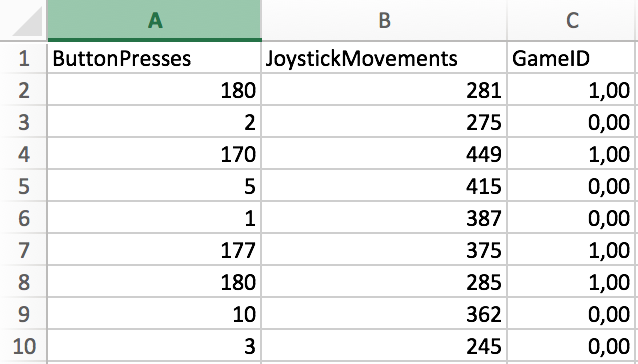
\includegraphics{img/Dataset}
	\caption{Tien voorbeelden van games}
	\label{fig:regressieFig}
\end{figure}


\newpage

\subsection{Logistische regressie}
\label{sec:Logistischeregressie-fase1}

Het eerste algoritme die we gaan testen is logistische regressie. In fase 1 gaan we slecht voorspellingen doen tussen twee verschillende spellen vandaar dat we binaire logistische regressie gaan toepassen die eerder uitgelegd is in sectie \ref{sec:Binaire-logistische-regressie}.

metaparameters die ervoor zorgen dat een algoritme stopt




\begin{lstlisting}
public static void StartLogisticRegression(double[][] input, int[] output)
{
       // Create a new Iterative Reweighted Least Squares algorithm
       LogisticRegression logisticRegression = new LogisticRegression()
       {
       		NumberOfInputs = 2
       };
      var learner = new LogisticGradientDescent(logisticRegression)
      {
      		Iterations = 100,
      		LearningRate = 0.0001
      };
            
     // Now, we can use the learner to finally estimate our model:
     logisticRegression = learner.Learn(input, output);

}

\end{lstlisting}
